\documentclass[12pt,a4paper]{article}
\usepackage[margin=1in]{geometry}
\usepackage{amsmath}
\usepackage{listings}
\usepackage{xcolor}
\usepackage{graphicx}

\begin{document}

\pagenumbering{gobble}

\section*{Playfair Cipher: Theoretical Overview}

The Playfair cipher, invented by Charles Wheatstone in 1854 and promoted by Lord Playfair, is a digraph substitution cipher. It encrypts pairs of letters, offering significant advantages over simple monoalphabetic substitution ciphers.

\subsection*{Features}
\begin{itemize}
    \item Uses a 5x5 grid of letters based on a keyword
    \item Encrypts digraphs (pairs of letters) instead of single letters
    \item 25 letters (I and J are typically combined)
    \item Resistant to frequency analysis attacks
\end{itemize}

\subsection*{Key Generation}
\begin{enumerate}
    \item Choose a keyword and remove duplicate letters
    \item Fill a 5x5 matrix with the keyword letters first
    \item Complete the matrix with remaining alphabet letters
    \item Example with keyword "MONARCHY":
    \[
    \begin{matrix}
    M & O & N & A & R \\
    C & H & Y & B & D \\
    E & F & G & I/J & K \\
    L & P & Q & S & T \\
    U & V & W & X & Z
    \end{matrix}
    \]
\end{enumerate}

\subsection*{Encryption Rules}
For each pair of plaintext letters $(a,b)$:
\begin{enumerate}
    \item If $a$ and $b$ are in the same row, replace with letters to their right (wrapping around)
    \item If $a$ and $b$ are in the same column, replace with letters below (wrapping around)
    \item Otherwise, replace with letters on the same row but in the column of the other letter
\end{enumerate}

% \subsection*{Mathematical Representation}
% Let $M$ be the key matrix, and $(i_1,j_1)$, $(i_2,j_2)$ be the positions of letters $a$ and $b$. The encryption function $E$ can be defined as:

% \[
% E(a,b) = \begin{cases}
%     (M_{i_1,(j_1+1)\mod 5}, M_{i_2,(j_2+1)\mod 5}) & \text{if } i_1 = i_2 \\
%     (M_{(i_1+1)\mod 5,j_1}, M_{(i_2+1)\mod 5,j_2}) & \text{if } j_1 = j_2 \\
%     (M_{i_1,j_2}, M_{i_2,j_1}) & \text{otherwise}
% \end{cases}
% \]

\subsection*{Security Considerations}
\begin{itemize}
    \item Stronger than simple substitution ciphers
    \item Vulnerable to known-plaintext attacks
    \item Frequency analysis of digraphs can be used for cryptanalysis
    \item Modern cryptography has rendered it obsolete for secure communication
\end{itemize}

% Define colors for syntax highlighting
\definecolor{codegreen}{rgb}{0,0.6,0}
\definecolor{codegray}{rgb}{0.5,0.5,0.5}
\definecolor{codepurple}{rgb}{0.58,0,0.82}
\definecolor{backcolour}{rgb}{0.95,0.95,0.92}

% \lstdefinestyle{mystyle}{
%     backgroundcolor=\color{backcolour},   
%     commentstyle=\color{codegreen},
%     keywordstyle=\color{magenta},
%     numberstyle=\tiny\color{codegray},
%     stringstyle=\color{codepurple},
%     basicstyle=\ttfamily\footnotesize,
%     breakatwhitespace=false,         
%     breaklines=true,                 
%     captionpos=t,                    
%     keepspaces=true,                 
%     numbers=left,                    
%     numbersep=5pt,                  
%     showspaces=false,                
%     showstringspaces=false,
%     showtabs=false,                  
%     tabsize=2,
%     language=Python
% }

% \lstset{style=mystyle}

\lstinputlisting[caption=playfair.py,language=Python,basicstyle=\ttfamily\footnotesize, captionpos=t, numbers=left, breaklines=true]{playfair.py}

\begin{figure}[h]
    \caption{Output}
    \centering
    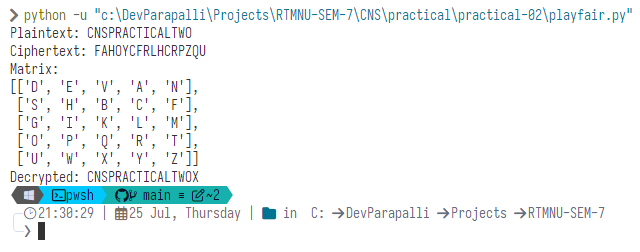
\includegraphics[width=\textwidth]{output.png}
\end{figure}

\newpage

% \begin{center}
%     \textbf{Output}
%     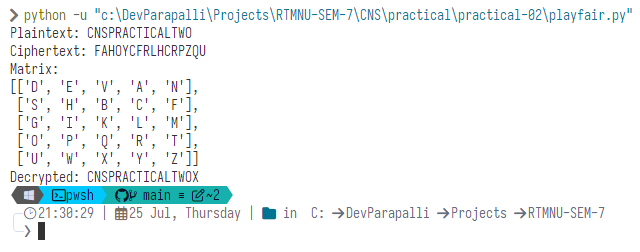
\includegraphics[width=\textwidth]{output.png}
% \end{center}

\end{document}